
\mychapter{Visão geral do MCTest}\label{ch:visaoGeral}

O MCTest é um sistema, gratuito, de código aberto e em desenvolvimento, cujo objetivo é fornecer e gerenciar um banco de dados para avaliações de estudantes em um sistema de ensino. O foco principal do sistema é fornecer questões que possam ser utilizadas em atividades de ensino, além de oferecer geração e correção automática de atividades e exames. Com o MCTest, os educadores terão acesso a uma ferramenta poderosa para avaliar o progresso dos estudantes, aprimorar o processo de ensino e fornecer \textit{feedback} de forma rápida.

O MCTest representa uma importante contribuição ao estado da arte em Tecnologia da Informação e Comunicação (TIC) ao fornecer métodos para a construção e correção automatizada de questões parametrizadas de múltipla escolha (QMs) e dissertativas (QTs). O sistema utiliza diferentes bibliotecas da linguagem de programação Python para calcular parâmetros na descrição e nas alternativas das questões de forma automática. Para mais detalhes, é possível consultar as publicações disponíveis em \href{http://vision.ufabc.edu.br}{vision.ufabc.edu.br}, algumas delas também serão apresentadas nos capítulos da Parte \ref{part:experimentos}. Além disso, o MCTest também suporta QTs que podem incluir exercícios de programação (EP) ou qualquer outro tipo de resposta.

O MCTest possui um ambiente de produção disponível em \href{http://mctest.ufabc.edu.br}{mctest.ufabc.edu.br}, atualmente utilizado por diversos professores e setores na Universidade Federal do ABC (UFABC). Por exemplo, a Escola Preparatória (EPUFABC) utiliza o sistema no processo seletivo anual de aproximadamente 3000 candidatos anualmente. Isso demonstra a eficácia e a confiabilidade do MCTest como uma ferramenta de avaliação em larga escala.

O MCTest está disponível gratuitamente no \href{http://github.com/fzampirolli/mctest}{GitHub}, permitindo que outras instituições possam copiar, personalizar e instalar o sistema em seus próprios servidores de forma livre e flexível. Além disso, há diversas possibilidades de melhoria e trabalhos futuros para o MCTest, as quais podem ser exploradas seguindo a filosofia de código aberto, como definido no \href{http://mctest.ufabc.edu.br/license}{Copyright © 2018–2023} do sistema. Para mais informações sobre as possibilidades de melhoria do MCTest, é possível consultar o \textit{link} \href{http://mctest.ufabc.edu.br/readme}{mctest.ufabc.edu.br/readme}.

\section{Navegação geral e usuários}

A navegação geral do MCTest visa possibilitar a criação e manutenção das entidades principais do sistema, que incluem instituto, curso, disciplina, turma, exame, tópico e questão. Os usuários do sistema são categorizados em três perfis: professor, coordenador e administrador. No entanto, na Figura \ref{fig:MCTest}, quando nenhum usuário está logado no sistema, um usuário da web pode visualizar os conteúdos públicos de institutos, cursos e disciplinas, bem como se inscrever ou entrar no sistema. Para uma comparação das funcionalidades de cada perfil de usuário, consulte também a Figura \ref{fig:cap2_navegacao}.
%
\begin{figure}[!ht]
  \centering
  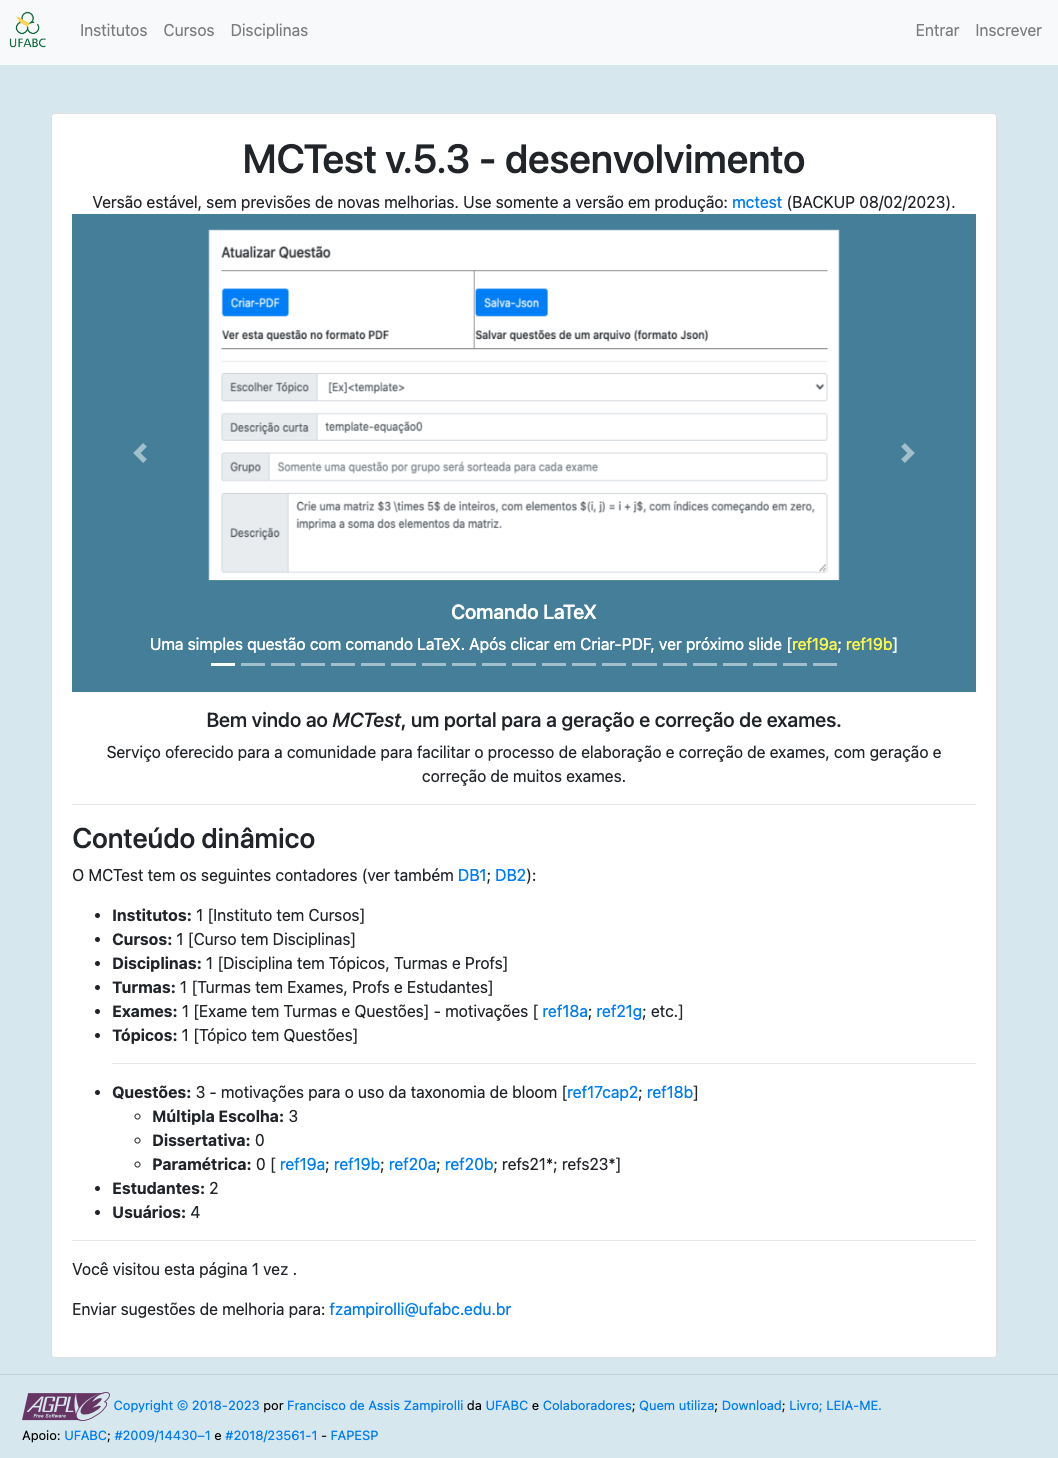
\includegraphics[width=0.9\textwidth]{cap02_figMCTest.png}
  \caption{Tela principal do MCTest.}
  \label{fig:MCTest}
\end{figure}


\begin{mybox}{corObs}{\textbf{Observação:\\\vspace{-3mm}\hrule\vspace{3mm}}}
As figuras apresentadas neste livro correspondem à implantação do MCTest em uma máquina local, utilizando um banco de dados de exemplo disponível no \href{https://github.com/fzampirolli/mctest}{GitHub}, com um número limitado de entidades cadastradas. Para ver um exemplo com um banco de dados mais completo, visite o site \href{http://mctest.ufabc.edu.br}{mctest.ufabc.edu.br}. Para adiantar, o leitor pode instalar uma máquina virtual utilizando o \href{https://www.virtualbox.org/}{VirtualBox} e, em seguida, fazer o \textit{download} de um sistema operacional suportado, conforme explicado no arquivo \href{https://github.com/fzampirolli/mctest/blob/master/_setup-all.sh}{\texttt{\_setup-all.sh}}. Basta seguir as instruções fornecidas nesse arquivo para concluir a instalação, incluindo a instalação das bibliotecas necessárias. É importante notar que o processo de instalação do pacote \LaTeX{} pode levar mais de 10 minutos. Para mais detalhes, ver Seção \ref{sec:instalacao} -- \nameref{sec:instalacao}.
\end{mybox}

Atualmente, além do administrador, o sistema está disponível apenas para usuários do tipo professor, que podem também ser coordenadores de disciplina com permissão para incluir professores e tópicos. O perfil de coordenador é adicionado pelo administrador do sistema ao associá-lo a uma disciplina específica. Cabe ao administrador também a responsabilidade de manter a página do \href{https://www.djangoproject.com/}{Django}.

No MCTest, cada tipo de usuário possui acesso restrito a um conjunto específico de entidades, como ilustrado na Figura \ref{fig:cap2_navegacao}. É importante ressaltar que os itens (c) e (d) são idênticos para professores e coordenadores. Por exemplo, ambos podem visualizar todas as turmas, tópicos e questões das disciplinas em que estão inscritos, mas somente o coordenador pode realizar alterações em tópicos de disciplinas que coordena. Além disso, os menus à esquerda são gerais para todo o conteúdo ao qual o usuário tem acesso, enquanto à direita são apresentados apenas os conteúdos de questões, turmas e exames que o usuário criou. 

\begin{figure}[!ht]
  \centering
  
\includegraphics[width=0.9\textwidth]{cap02_figNavega01.png} 
  \\ (a) Navegação sem estar logado \\ 
  
\includegraphics[width=0.9\textwidth]{cap02_figNavega02.png}
  \\ (b) Navegação para um usuário cadastrado sem perfil \\   
  
\includegraphics[width=0.9\textwidth]{cap02_figNavega03.png}
  \\ (c) Navegação para um usuário com perfil de professor \\ 
  
\includegraphics[width=0.9\textwidth]{cap02_figNavega04.png}
  \\ (d) Navegação para um usuário com perfil de coordenador \\ 
  
\includegraphics[width=0.9\textwidth]{cap02_figNavega05.png}
  \\ (e) Navegação para um usuário com perfil de administrador \\ 
  \caption{Recorte do menu de navegação principal do MCTest.}
  \label{fig:cap2_navegacao}
\end{figure}

O MCTest também permite que um professor coordenador de disciplina adicione vários professores a uma disciplina por um arquivo CSV, sendo automaticamente cadastrado no sistema como perfil de professor (esse processo será exemplificado no próximo capítulo). Com isso, os professores incluídos na disciplina têm acesso somente às funcionalidades do sistema que são relevantes ao seu perfil.

\begin{mybox}{corEdicao2}{\textbf{Destaque:\\\vspace{-3mm}\hrule\vspace{3mm}}}
Para enfatizar um ponto específico no que se refere ao registro de professores, é de extrema relevância ressaltar que, quando um professor efetua seu cadastro de forma independente, ele não é automaticamente incluído no grupo de professores. Nessa situação, torna-se imperativo que um administrador intervenha a fim de efetuar essa inclusão, por meio do acesso à aba ``Admin'', conforme ilustrado na Figura \ref{fig:cap2_navegacao}-(e).
\end{mybox}

Antes de demonstrar como criar entidades no sistema, é importante cadastrar-se na plataforma, clicando na opção ``Inscrever'', conforme indicado na Figura \ref{fig:cap2_navegacao} e exemplificado na Figura \ref{fig:inscrever}. É necessário ressaltar que somente os professores podem se inscrever neste serviço e devem utilizar o e-mail institucional fornecido pela instituição durante o cadastro. Por exemplo, o endereço \texttt{user@ufabc.edu.br} é válido, enquanto \texttt{user@aluno.ufabc.edu.br} é inválido. O e-mail deve conter a URL da instituição (por exemplo, \texttt{@ufabc.edu.br}). Tais restrições são cruciais para garantir a validade e a segurança das informações associadas às instituições cadastradas no sistema. Finalmente, o botão ``De Acordo'', apresentado na Figura \ref{fig:inscrever}, foi detalhado na Seção \ref{sec:deAcordo} -- \nameref{sec:deAcordo}.

\begin{mybox}{pink}{\textbf{Melhorias:\\\vspace{-3mm}\hrule\vspace{1mm}}}
\begin{itemize}
    \item É importante ressaltar que ainda não foi implementada a funcionalidade de segurança para validar o e-mail durante o processo de inscrição. Será necessário implementar essa funcionalidade para garantir a integridade e a segurança dos dados cadastrados no sistema.
    \item Outra melhoria importante para a segurança do sistema é a utilização de um certificado digital, que permitirá a utilização do protocolo HTTPS em vez de HTTP nos servidores utilizados para a implantação do MCTest. O HTTPS criptografa a comunicação entre o navegador do usuário e o servidor, garantindo a confidencialidade e a integridade dos dados transmitidos. 
\end{itemize}
\end{mybox}

\begin{figure}[!ht]
  \centering
  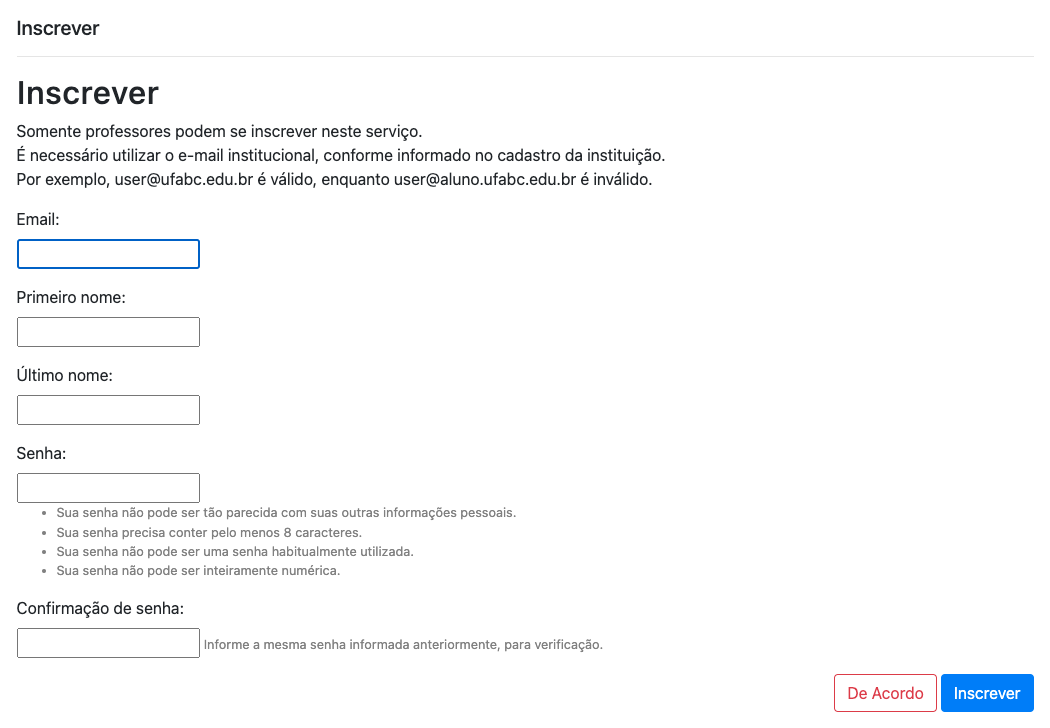
\includegraphics[width=0.9\textwidth]{cap02_figInscrever.png} 
  \caption{Tela para a inscrição do usuário.}
  \label{fig:inscrever}
\end{figure}

\section{Criar entidades}

O MCTest é um sistema que gerencia diversas entidades em um banco de dados MySQL, como detalhado neste e no próximo capítulo. Essas entidades são criadas e relacionadas para modelar o domínio educacional com foco na avaliação dos estudantes. Além disso, o sistema oferece funcionalidades para o cadastro, alteração, remoção e consulta dessas entidades e seus relacionamentos.

Nesta seção, você encontrará a descrição das principais entidades de negócio de um sistema educacional que tem como foco as avaliações. É importante ressaltar que, embora as entidades, questão e exame sejam de extrema importância no contexto do MCTest, elas serão abordadas em capítulos específicos para uma exposição mais detalhada e aprofundada.

\subsection{Instituto}\label{sec:instituto}

A entidade instituto representa a instituição cadastrada no sistema e contém atributos como nome, código, logo, site, entre outros.
%
A criação de uma entidade instituto é restrita ao usuário com perfil de administrador. 

Na Figura \ref{fig:instituto}, ao clicar em ``Criar um novo Instituto'', uma tela será aberta para cadastrar informações sobre o instituto, conforme ilustrado na Figura \ref{fig:cap02_figInstitutoCria}. Ao clicar em um instituto existente na coluna ``Código'' ou ``Nome'' da Figura \ref{fig:instituto}, o usuário será direcionado para uma tela para visualizar as informações do instituto, conforme ilustrado na Figura \ref{fig:cap02_figInstitutoDetalha}. É importante observar que nesta tela também é apresentada a lista de cursos, que será detalhada na próxima seção. 

Ao clicar no botão ``Atualizar'' em um instituto existente na coluna ``Ações'' da Figura \ref{fig:instituto}, o usuário será direcionado para uma nova tela para atualizá-lo, semelhante à Figura \ref{fig:cap02_figInstitutoCria}. Se o usuário clicar em ``Apagar'', o instituto será removido do banco de dados, após confirmação na janela de diálogo apresentada na Figura \ref{fig:cap02_figInstitutoRemover}.


\begin{figure}[!ht]
  \centering
  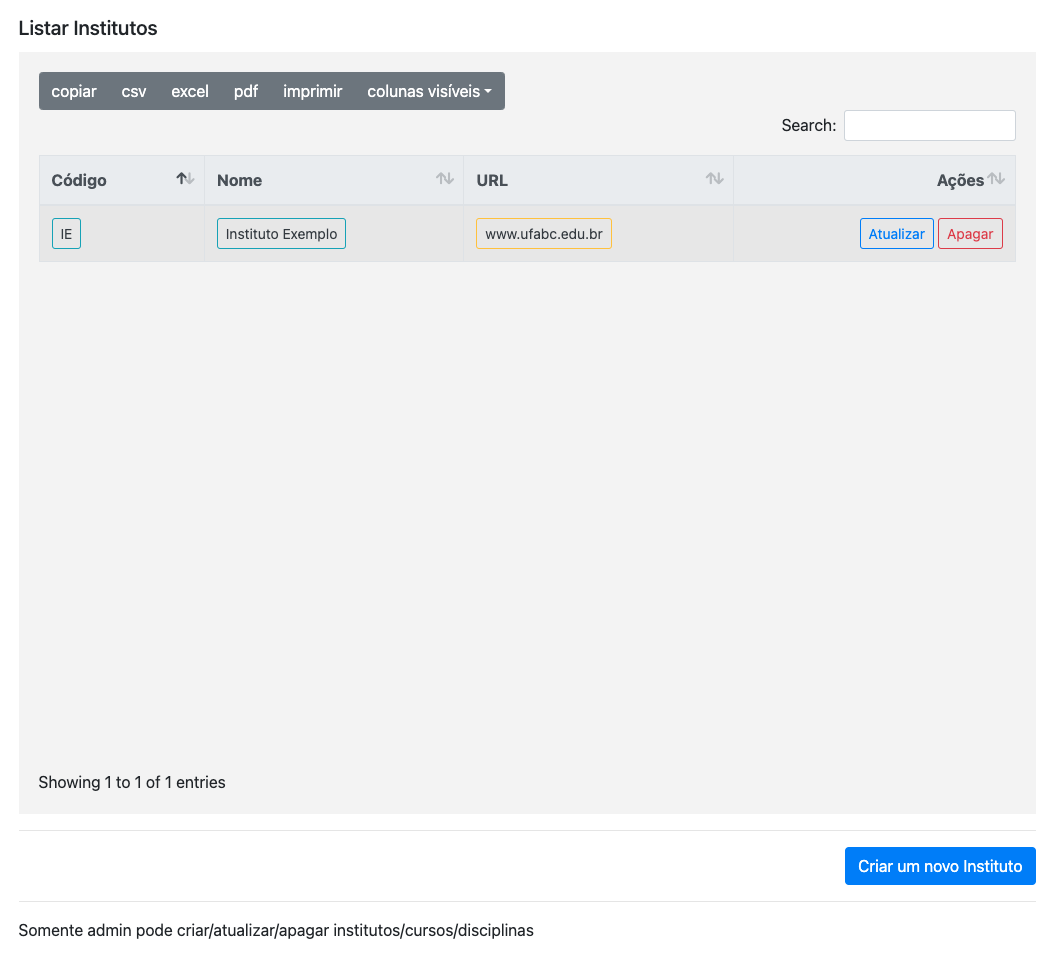
\includegraphics[width=0.9\textwidth]{cap02_figInstituto.png}
  \caption{Tela para administrador atualizar, apagar ou criar um instituto.}
  \label{fig:instituto}
\end{figure}

A Figura \ref{fig:cap02_figInstitutoCria} apresenta o recorte da tela para ``Criar de um novo Instituto'', que é similar à de ``Atualizar um Instituto''. Os três últimos campos exibidos na tela são utilizados para contabilizar o número de exames e questões gerados e corrigidos pelo sistema desde a criação do instituto. Esses contadores são úteis para monitorar a atividade do sistema em relação a cada instituto.
%
É importante ressaltar que apenas o administrador pode zerar esses contadores a qualquer momento, o que pode ser necessário em algumas circunstâncias, como quando é necessário reiniciar as contagens ou avaliar a atividade recente do sistema.

\begin{figure}[!ht]
  \centering
  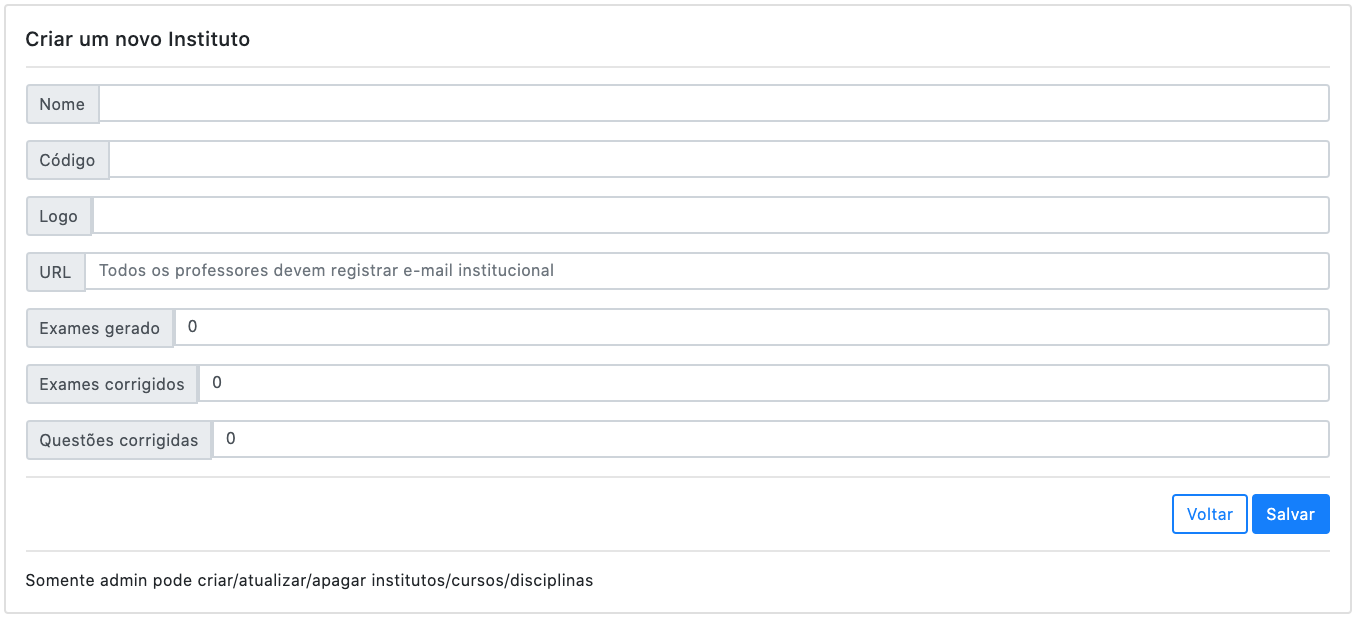
\includegraphics[width=0.9\textwidth]{figs-br/cap02_figInstitutoCria.png}
  \caption{Tela para o administrador criar um instituto.}
  \label{fig:cap02_figInstitutoCria}
\end{figure}


\begin{mybox}{corObs}{\textbf{Observação:\\\vspace{-3mm}\hrule\vspace{3mm}}}
As telas e as ações de criar, ler, atualizar e remover (CRUD -- \textit{Create, Read, Update, Delete}) para fazer a manutenção do instituto são semelhantes, em geral, às demais entidades do MCTest. Portanto, a partir deste ponto, serão apresentadas apenas as telas com informações diferentes, para o usuário poder se concentrar nas especificidades da manutenção das entidades do sistema.
Além disso, os nomes dessas entidades nessas telas devem seguir o formato \LaTeX.
\end{mybox}


\begin{figure}[!ht]
  \centering
  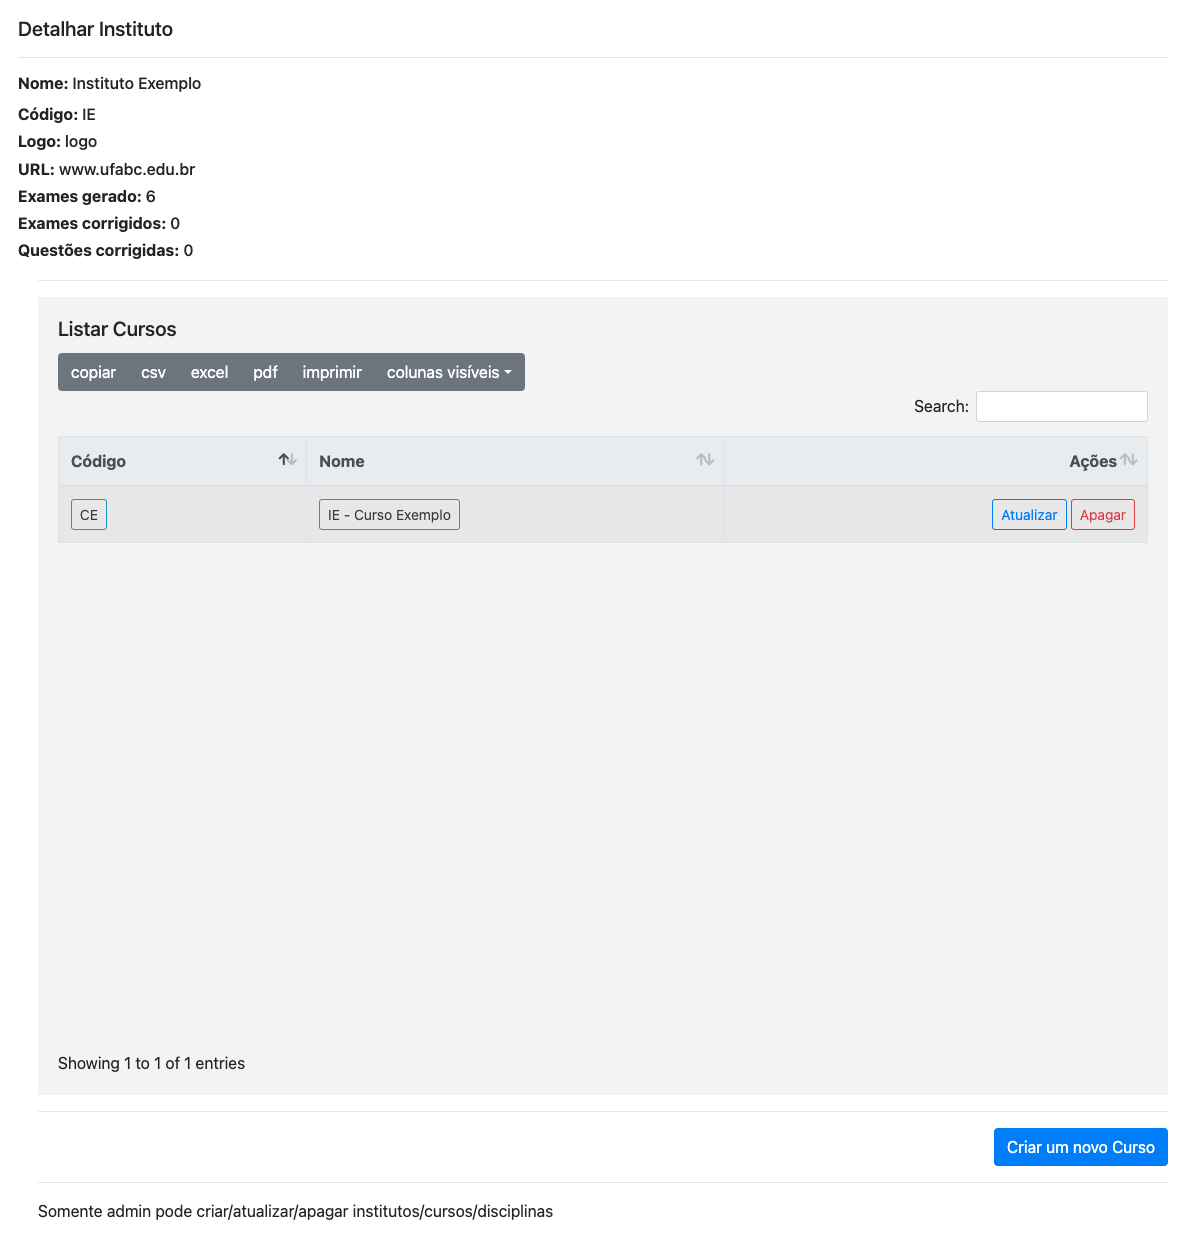
\includegraphics[width=0.9\textwidth]{cap02_figInstitutoDetalha.png}
  \caption{Tela apresentando os detalhes de um instituto.}
  \label{fig:cap02_figInstitutoDetalha}
\end{figure}

\begin{figure}[!ht]
  \centering
  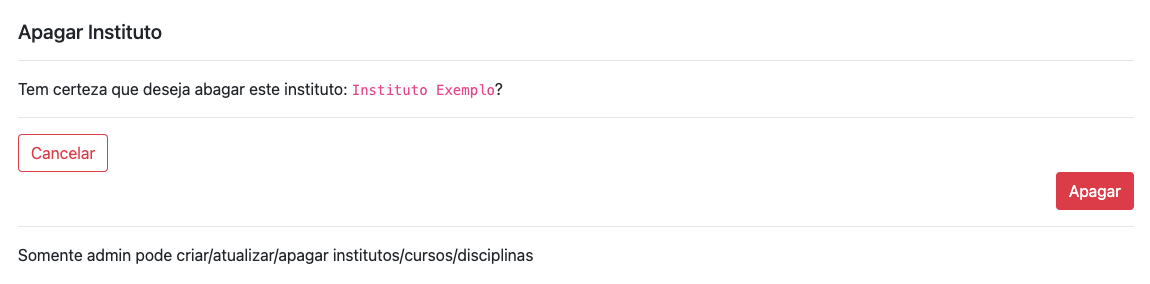
\includegraphics[width=0.9\textwidth]{cap02_figInstitutoRemover.png}
  \caption{Tela para confirmar a exclusão do instituto.}
  \label{fig:cap02_figInstitutoRemover}
\end{figure}

% \newpage

% \ \\ \ 

% \newpage

% \ \\ \ 

% \newpage

\subsection{Curso}\label{sec:curso}

A criação da entidade curso é restrita ao usuário com perfil de administrador, como ilustrado na Figura \ref{fig:curso}, que também pode atualizar ou apagar um curso existente, conforme apresentado na coluna ``Ações'' (outros tipos de usuários não têm acesso a esses botões). É importante destacar que um curso pode pertencer a um ou vários institutos, permitindo assim a organização dos cursos de acordo com sua área de atuação ou afinidade temática.

Na UFABC, por exemplo, um instituto como o Centro de Matemática, Computação e Cognição (CMCC) pode conter vários cursos. Além disso, um curso pode pertencer a mais de um instituto, e existem também cursos intercentros, como o Bacharelado em Ciência e Tecnologia (BCT), que pode pertencer ao instituto PROGRAD (Pró-Reitoria de Graduação) e também aos três centros existentes na UFABC.

Outros exemplos de cursos na UFABC incluem a Escola Preparatória, que pode ser um curso do instituto PROEC (Pró-Reitoria de Extensão e Cultura), e o curso de idiomas, que pertence ao instituto NETEL (Núcleo Educacional de Tecnologias e Línguas), entre outros. 

\begin{figure}[!ht]
  \centering
  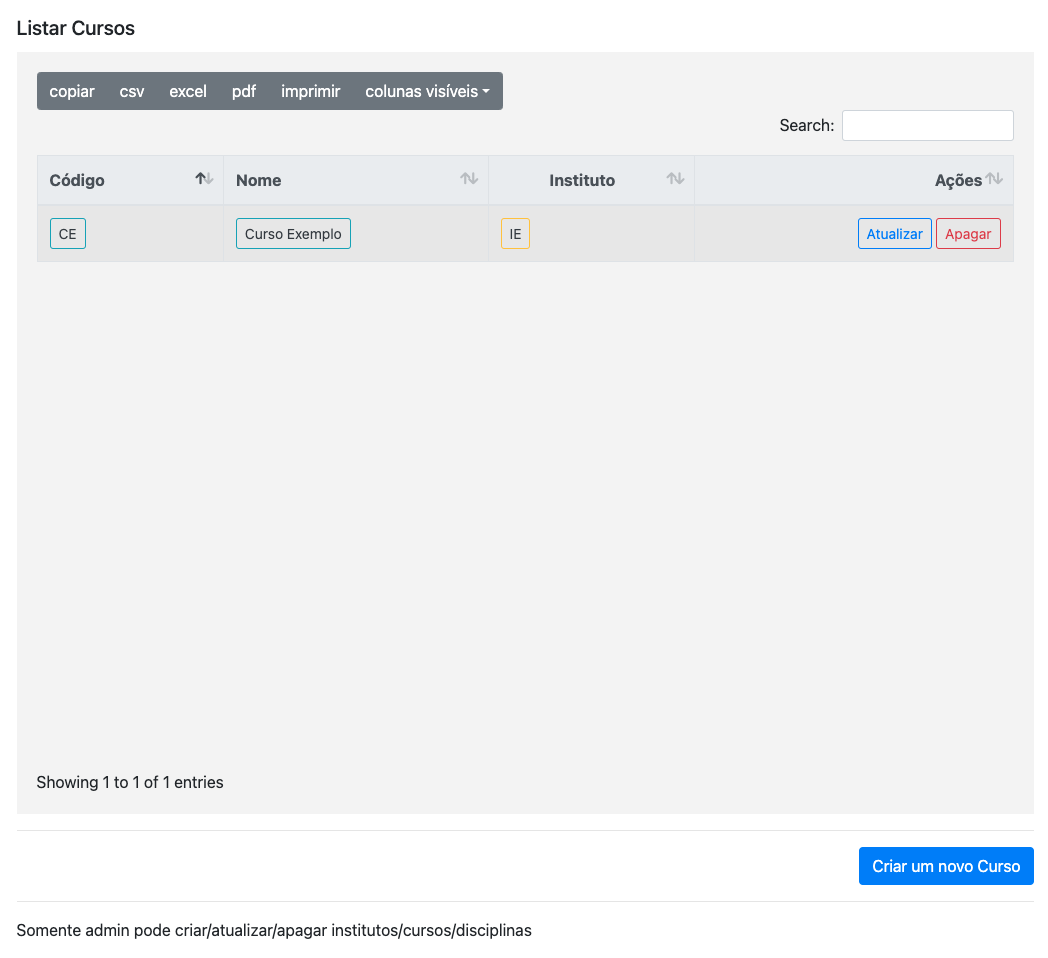
\includegraphics[width=0.9\textwidth]{cap02_figCurso.png}
  \caption{Tela que apresenta a lista de cursos, na qual o administrador pode atualizar, apagar ou criar um novo curso.}
  \label{fig:curso}
\end{figure}

Essa flexibilidade na associação dos cursos aos institutos permite uma maior customização do sistema de avaliação educacional do MCTest, conforme as necessidades específicas de cada instituição ou curso. Dessa forma, é possível adaptar o sistema para atender às demandas e particularidades de diferentes áreas de conhecimento e instituições de ensino.

Ao clicar no botão ``Criar um novo Curso'' na Figura \ref{fig:curso}, o administrador será direcionado para a tela de criação de um novo curso, apresentada na Figura \ref{fig:cursoCria}. Nesta tela, o administrador deve preencher as informações necessárias sobre o curso, como o nome e código. Além disso, é necessário selecionar o instituto ao qual o curso pertence, como exemplificado no caso do ``Instituto Exemplo''. É importante destacar que é possível associar mais de um instituto a um curso específico, como será exemplificado no próximo capítulo. Após preencher todas as informações, o administrador deve clicar no botão ``Salvar'' para salvar o curso no banco de dados do sistema.

\begin{figure}[!ht]
  \centering
  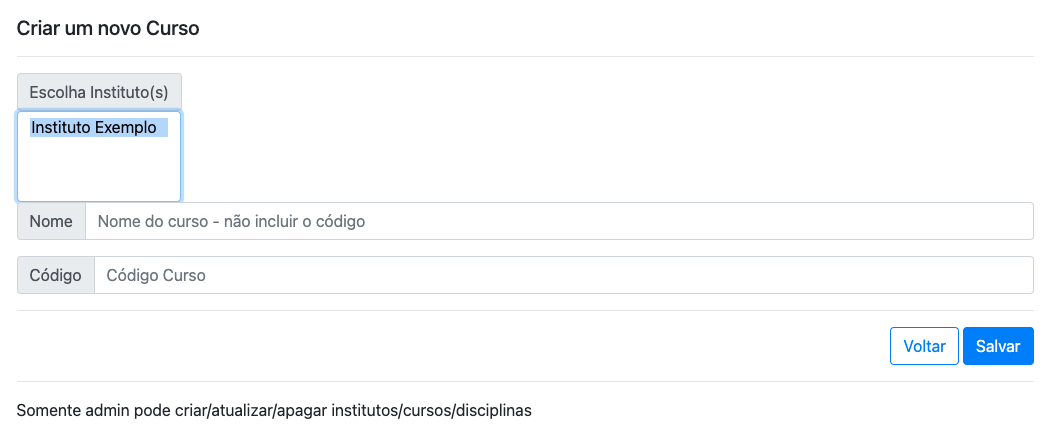
\includegraphics[width=0.9\textwidth]{cap02_figCursoCria.png}
  \caption{Tela para administrador criar um curso novo.}
  \label{fig:cursoCria}
\end{figure}

\begin{mybox}{pink}{\textbf{Melhorias:\\\vspace{-3mm}\hrule\vspace{3mm}}}
   É importante destacar que o banco de dados do sistema já suporta o relacionamento entre um conjunto de professores/coordenadores e uma instituição/curso. Portanto, é necessário implementar as funcionalidades que permitam vincular esses profissionais às entidades correspondentes. Isso permitirá que a gestão dos professores/coordenadores seja feita de forma mais organizada e eficiente, facilitando a alocação desses profissionais em diferentes cursos ou instituições. 
\end{mybox}


Ao clicar em um curso nas colunas ``Código'' ou ``Nome'' na Figura \ref{fig:curso}, o usuário será direcionado para uma tela detalhando as informações do curso selecionado, conforme ilustrado na Figura \ref{fig:cap02_figCursoDetalha}. É importante observar que nesta tela também são inseridas informações sobre as disciplinas do curso selecionado, em forma de uma lista. A manutenção das disciplinas será abordada na próxima seção.

\begin{figure}[!ht]
  \centering
  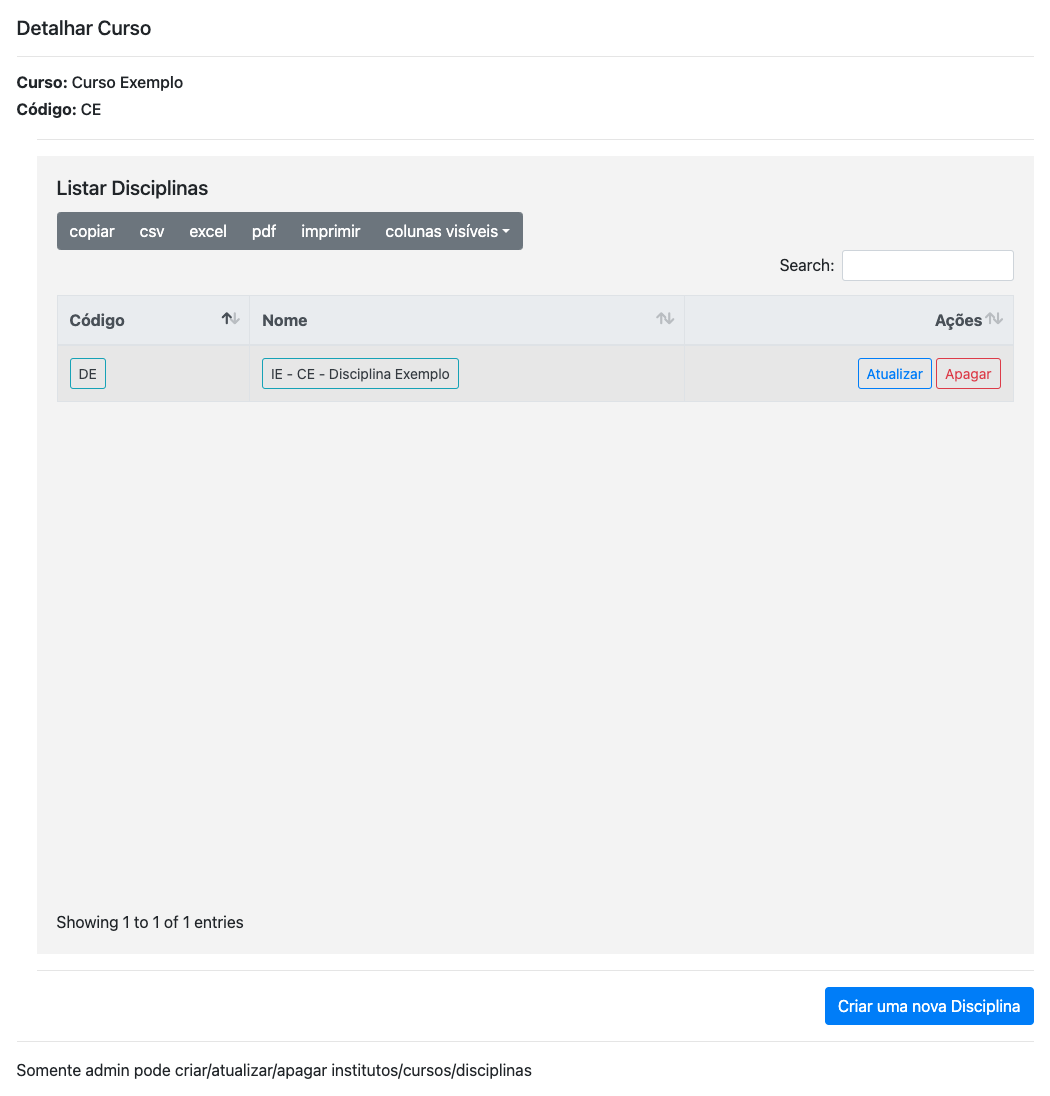
\includegraphics[width=0.9\textwidth]{cap02_figCursoDetalha.png}
  \caption{Tela apresentando os detalhes de um curso.}
  \label{fig:cap02_figCursoDetalha}
\end{figure}

% \newpage

% \ \\ \ 

% \newpage

% \ \\ \ 

\subsection{Disciplina}\label{sec:disciplina}

A entidade disciplina é responsável por representar as disciplinas cadastradas no sistema, sendo sua criação restrita ao usuário com perfil de administrador, que também pode atualizar ou apagar uma disciplina existente, como ilustrado na Figura \ref{fig:cap02_figDisciplina}, conforme apresentado na coluna ``Ações'' (outros tipos de usuários não têm acesso a esses botões de ação). No entanto, o usuário com perfil de coordenador possui permissão apenas para atualizar a disciplina que coordena, como será detalhado na próxima seção.

A entidade disciplina é essencial para a organização das turmas e tópicos, o que permite criar exames específicos para atender a várias turmas simultaneamente, facilitando a gestão e a aplicação de avaliações na plataforma.

\begin{figure}[!ht]
  \centering
  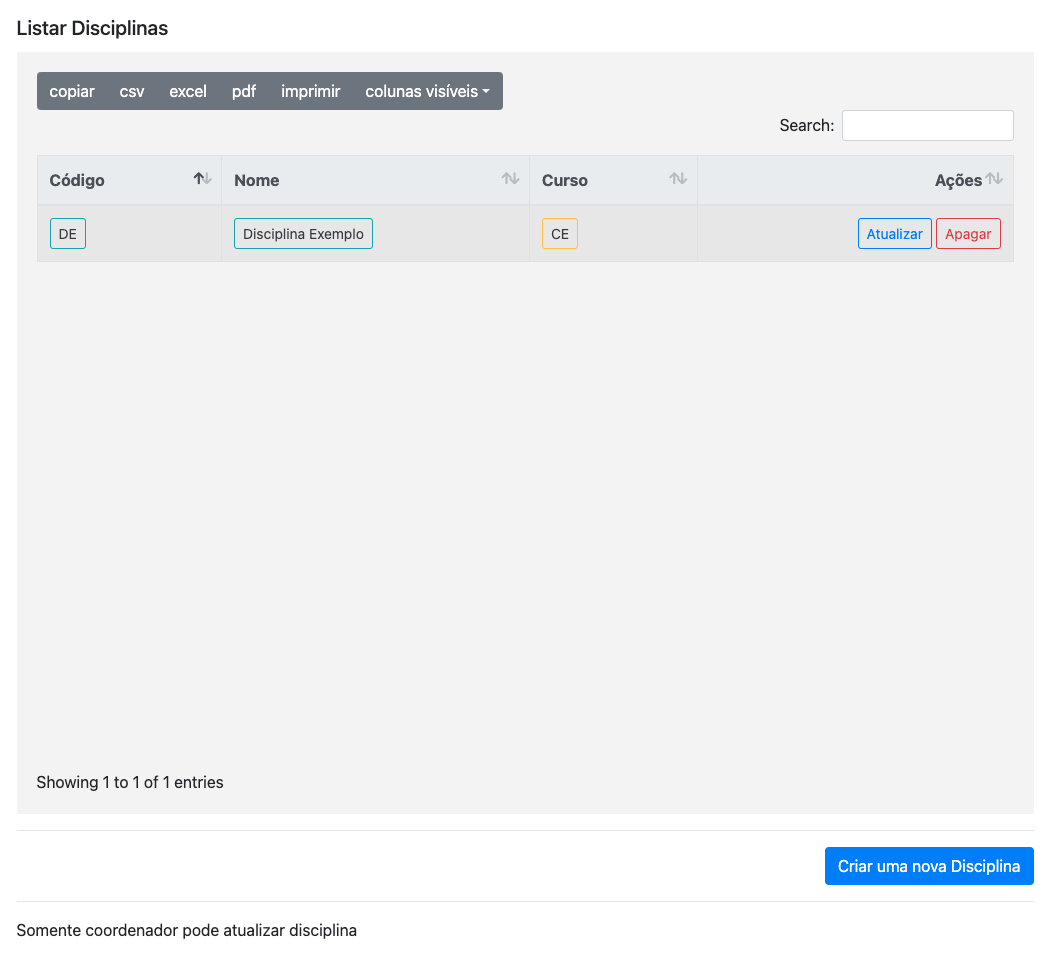
\includegraphics[width=0.9\textwidth]{cap02_figDisciplina.png}
  \caption{Tela que apresenta a lista de disciplinas, na qual o administrador pode atualizar, apagar ou criar uma nova disciplina.}
  \label{fig:cap02_figDisciplina}
\end{figure}

A Figura \ref{fig:cap02_figDisciplinaCria} mostra a tela para criar uma disciplina. Esta tela é semelhante à primeira parte da tela de atualização de uma disciplina. No caso de uma disciplina com muitas turmas, foram implementadas funcionalidades na segunda parte da tela de atualização de disciplina para o coordenador poder cadastrar todos os professores e estudantes de várias turmas de uma só vez, através da importação de arquivos no formato CSV, conforme ilustrado na Figura \ref{fig:cap02_figDisciplinaAtualiza22}. Essa funcionalidade será detalhada no próximo capítulo, na Seção \ref{sec:variasTurmasCSV}  -- \nameref{sec:variasTurmasCSV}.

A flexibilidade na associação de cursos permite uma personalização maior do sistema de avaliação educacional do MCTest, conforme as necessidades específicas de cada disciplina. Além disso, é possível associar professores e coordenadores à disciplina, permitindo uma organização mais eficiente e atribuição de responsabilidades na gestão da disciplina. Para selecionar mais de um professor, basta manter a tecla \textbf{Ctrl} pressionada.

É fundamental destacar que a criação e associação de disciplinas aos cursos devem ser realizadas com cautela e atenção pelo coordenador, visando garantir a precisão e efetividade da avaliação educacional. A associação correta de disciplinas aos respectivos cursos, institutos e professores é crucial para a realização de exames precisos e eficazes.

\begin{figure}[!ht]
  \centering
  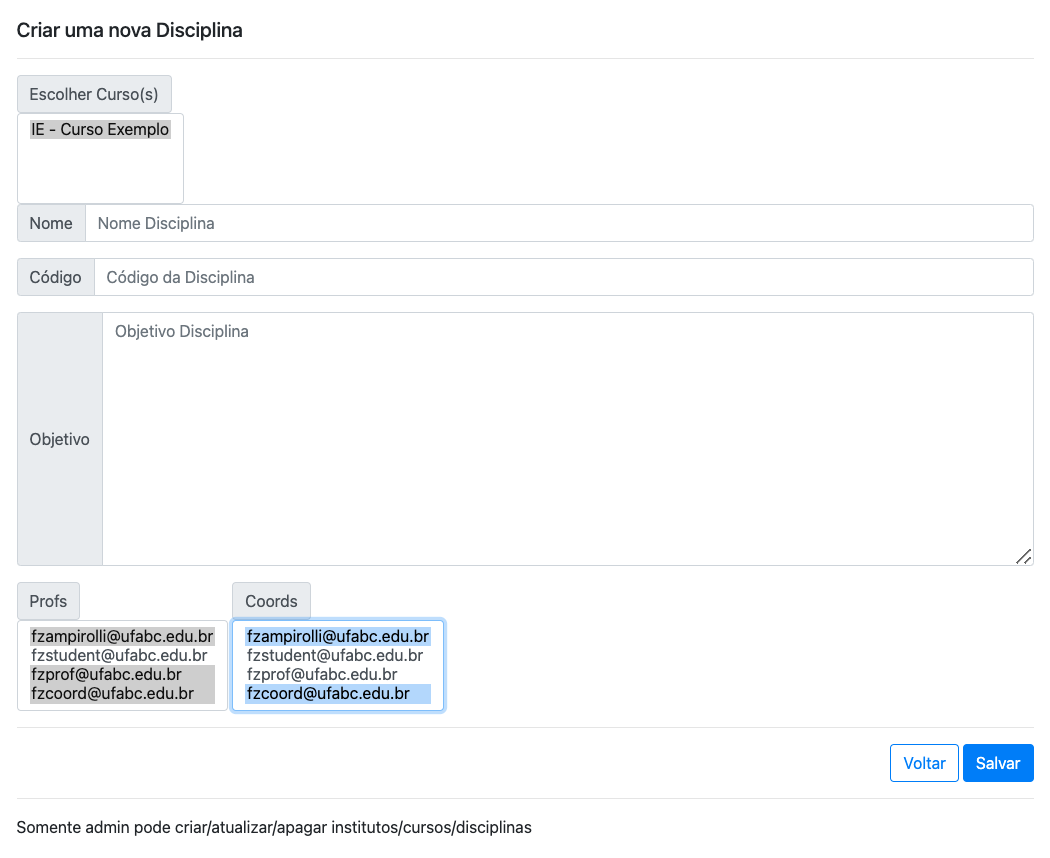
\includegraphics[width=0.9\textwidth]{cap02_figDisciplinaCria.png}
  \caption{Tela para o administrador criar uma disciplina. Tela semelhante à primeira parte da tela de atualizar uma disciplina.}
  \label{fig:cap02_figDisciplinaCria}
\end{figure}

\begin{figure}[!ht]
  \centering
  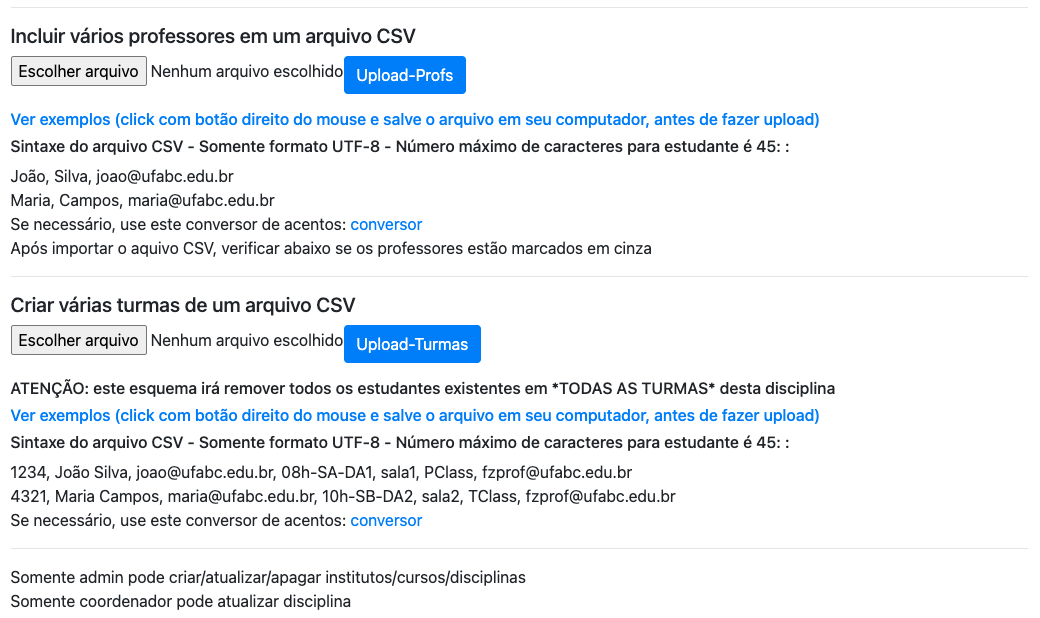
\includegraphics[width=0.9\textwidth]{cap02_figDisciplinaAtualiza2.png}
  \caption{Segunda parte da tela para o administrador atualizar uma disciplina.}
  \label{fig:cap02_figDisciplinaAtualiza22}
\end{figure}

Ao clicar em uma disciplina nas colunas ``Código'' ou ``Nome'' da Figura \ref{fig:cap02_figDisciplina}, será aberta uma tela detalhando as informações da disciplina, conforme ilustrado nas Figuras \ref{fig:cap02_figDisciplinaDetalha} e \ref{fig:cap02_figDisciplinaDetalha2}.

\begin{figure}[!ht]
  \centering
  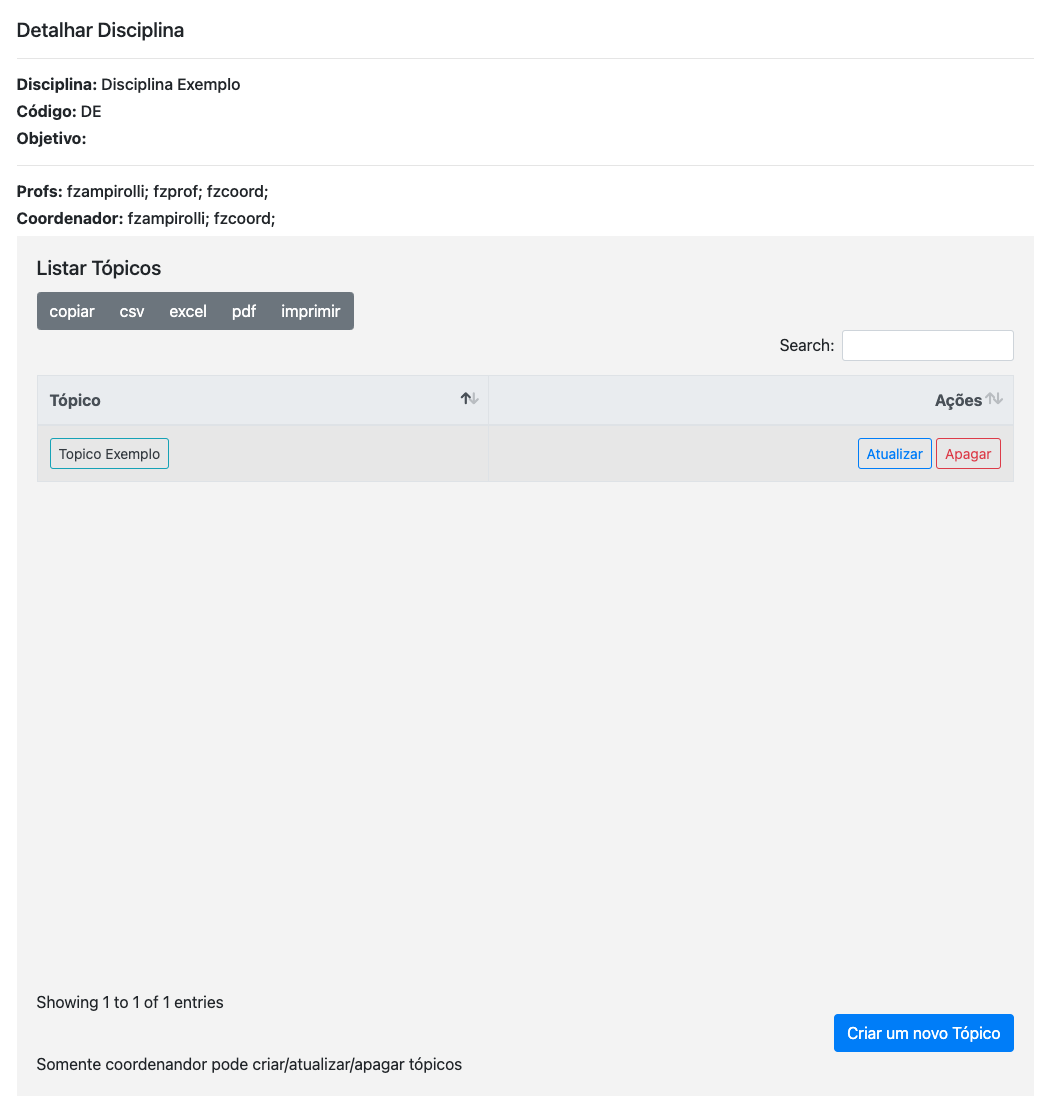
\includegraphics[width=0.9\textwidth]{cap02_figDisciplinaDetalha.png}
  \caption{(Parte 1) Tela apresentando os detalhes de uma disciplina.}
  \label{fig:cap02_figDisciplinaDetalha}
\end{figure}

\begin{figure}[!ht]
  \centering
  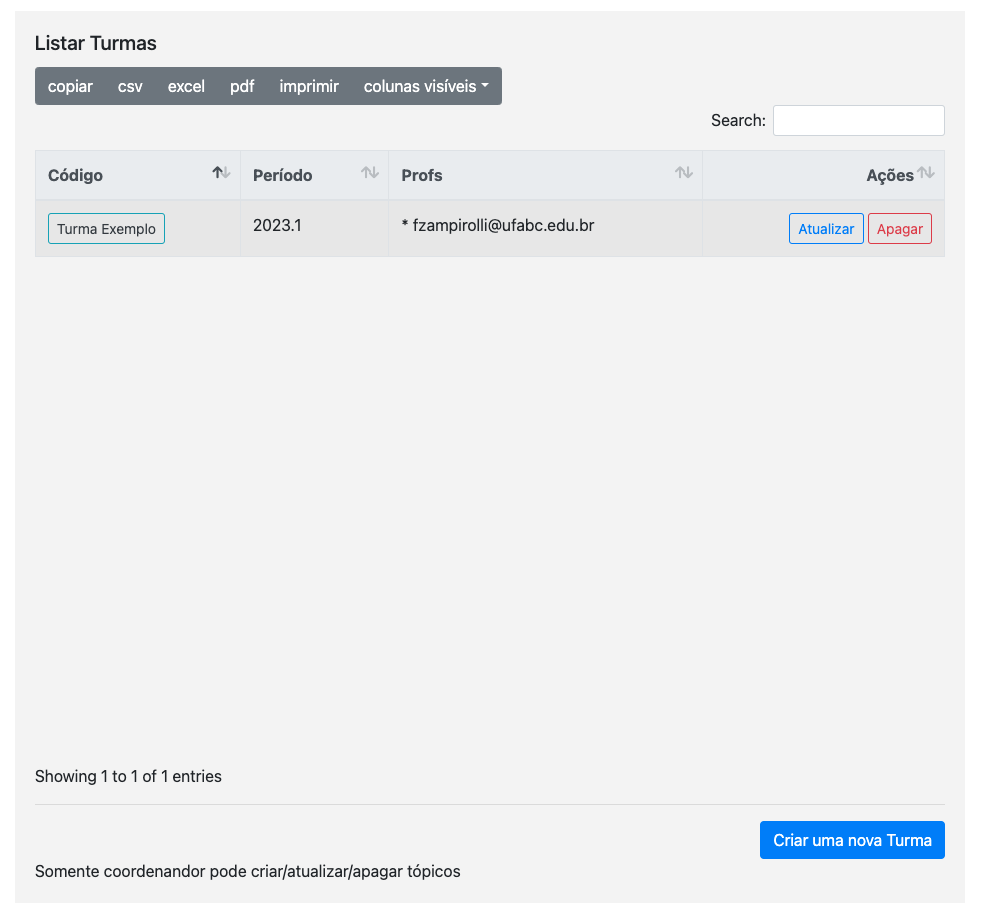
\includegraphics[width=0.9\textwidth]{cap02_figDisciplinaDetalha2.png}
  \caption{(Parte 2) Continuação da tela apresentando os detalhes de uma disciplina.}
  \label{fig:cap02_figDisciplinaDetalha2}
\end{figure}

% \newpage

% \ \\ \ 

% \newpage

% \ \\ \ 

% \newpage

% \ \\ \ 

% \newpage

% \ \\ \ 

% \newpage

% \ \\ \ 

\subsection{Turma}\label{sec:turma}

A entidade turma é responsável por representar as turmas cadastradas para cada disciplina no MCTest. A criação, atualização ou exclusão de turmas pode ser realizada pelo administrador, pelo coordenador ou pelo professor da disciplina, conforme apresentado na Figura \ref{fig:cap02_figTurma}. Nesta figura, o professor tem a opção de criar uma nova turma ao clicar em ``Criar uma nova Turma'', abrindo a tela apresentada na Figura \ref{fig:cap02_figTurmaCriar}. Para isso, é necessário escolher uma disciplina, definir o código da sala da disciplina e especificar se a turma é de teoria ou prática.

\begin{figure}[!ht]
  \centering
  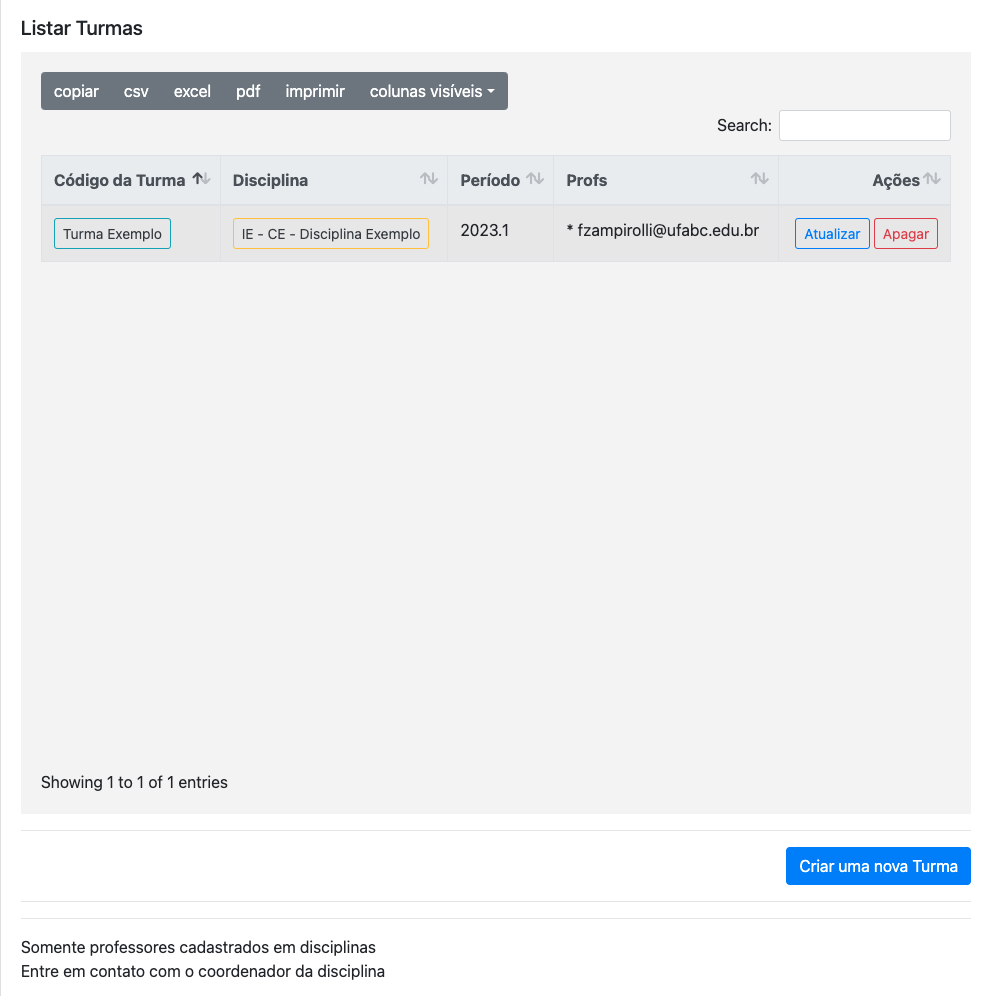
\includegraphics[width=0.9\textwidth]{cap02_figTurma.png}
  \caption{Tela que apresenta a lista de turmas, na qual um professor de uma disciplina pode criar uma nova turma, além de atualizar ou apagar turmas existentes.}
  \label{fig:cap02_figTurma}
\end{figure}



\begin{figure}[!ht]
  \centering
  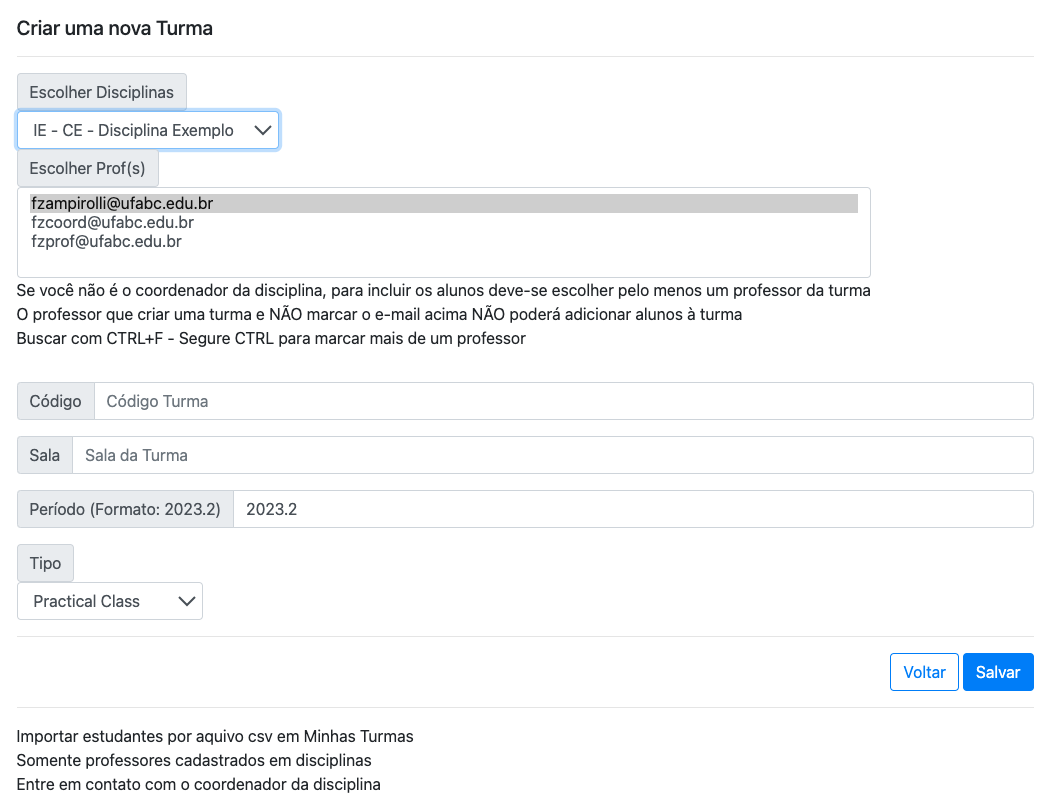
\includegraphics[width=0.9\textwidth]{cap02_figTurmaCriar.png}
  \caption{Tela utilizada pelo professor para criar uma nova turma após clicar no botão ``Criar uma nova Turma'', na tela da Figura \ref{fig:cap02_figTurma}. É importante destacar que o nome da turma não pode conter acentos ou caracteres especiais, pois esse nome fará parte do cabeçalho do exame.}
  \label{fig:cap02_figTurmaCriar}
\end{figure}

Após a criação da turma pelo professor, a tela apresentada na Figura \ref{fig:cap02_figTurma} deve ser atualizada e é possível clicar em ``Atualizar'' na coluna ``Ações'' para inserir estudantes na turma. Essa ação levará à tela de atualização da turma, conforme ilustrado na Figura \ref{fig:cap02_figTurmaAtualiza}. Nessa tela, é possível fazer a importação de um arquivo no formato CSV contendo a lista de estudantes que serão adicionados à turma.

\begin{figure}[!ht]
  \centering
  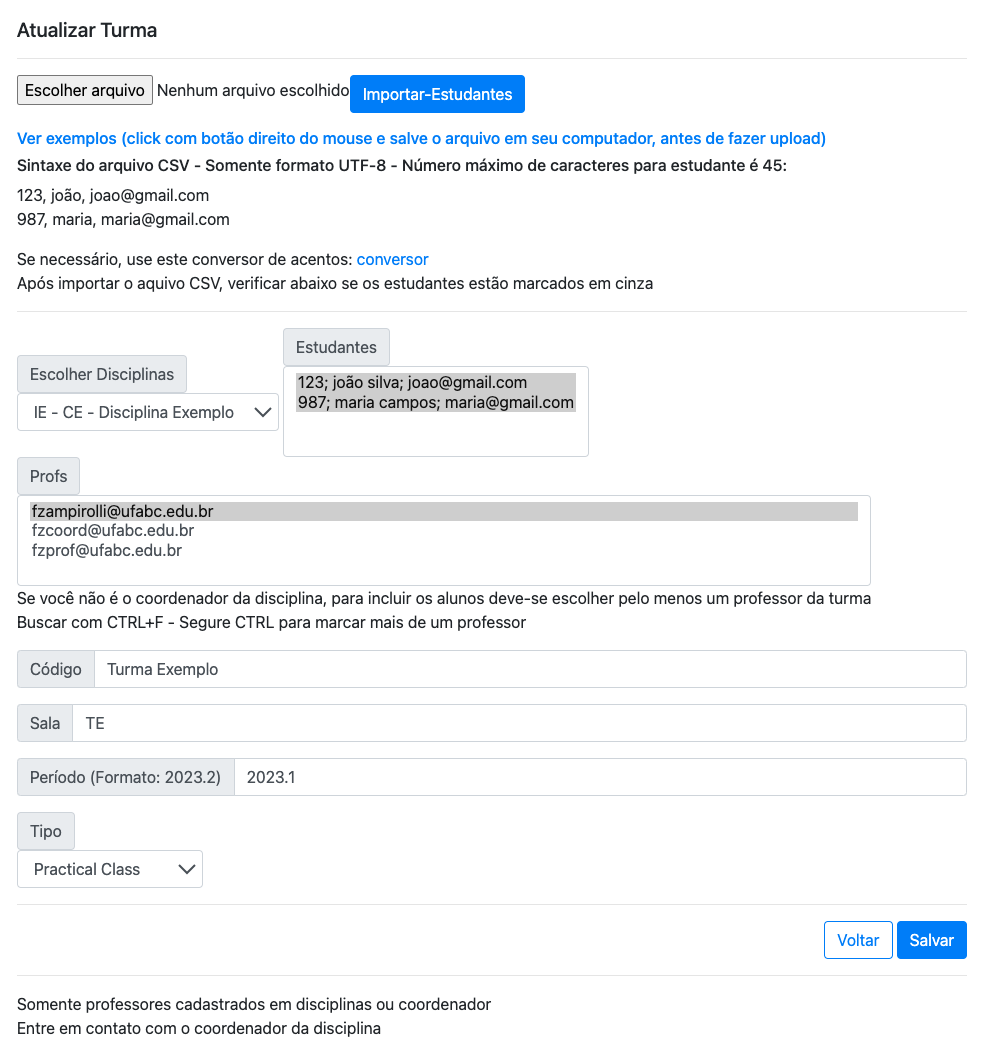
\includegraphics[width=0.9\textwidth]{cap02_figTurmaAtualiza.png}
  \caption{Tela para um professor de uma disciplina poder atualizar uma turma, inserindo estudantes com a importação de um arquivo no formato CSV.}
  \label{fig:cap02_figTurmaAtualiza}
\end{figure}

Na Figura \ref{fig:cap02_figTurma}, o professor pode clicar no código da turma (primeira coluna) e aparece a tela apresentada na Figura \ref{fig:cap02_figTurmaAtualiza2}, onde o professor pode atualizar ou apagar estudantes. Veja na Figura \ref{fig:cap02_figTurmaAtualiza3} a tela para atualizar os dados de um estudante.

Na Figura \ref{fig:cap02_figTurmaAtualiza}, é possível observar uma lista de todas as disciplinas do professor, se houver alguma, em ``Escolher Disciplinas''. Ao clicar no código de uma turma específica (primeira coluna), o professor pode acessar a tela apresentada na Figura \ref{fig:cap02_figTurmaAtualiza2}.


\begin{figure}[!ht]
  \centering
  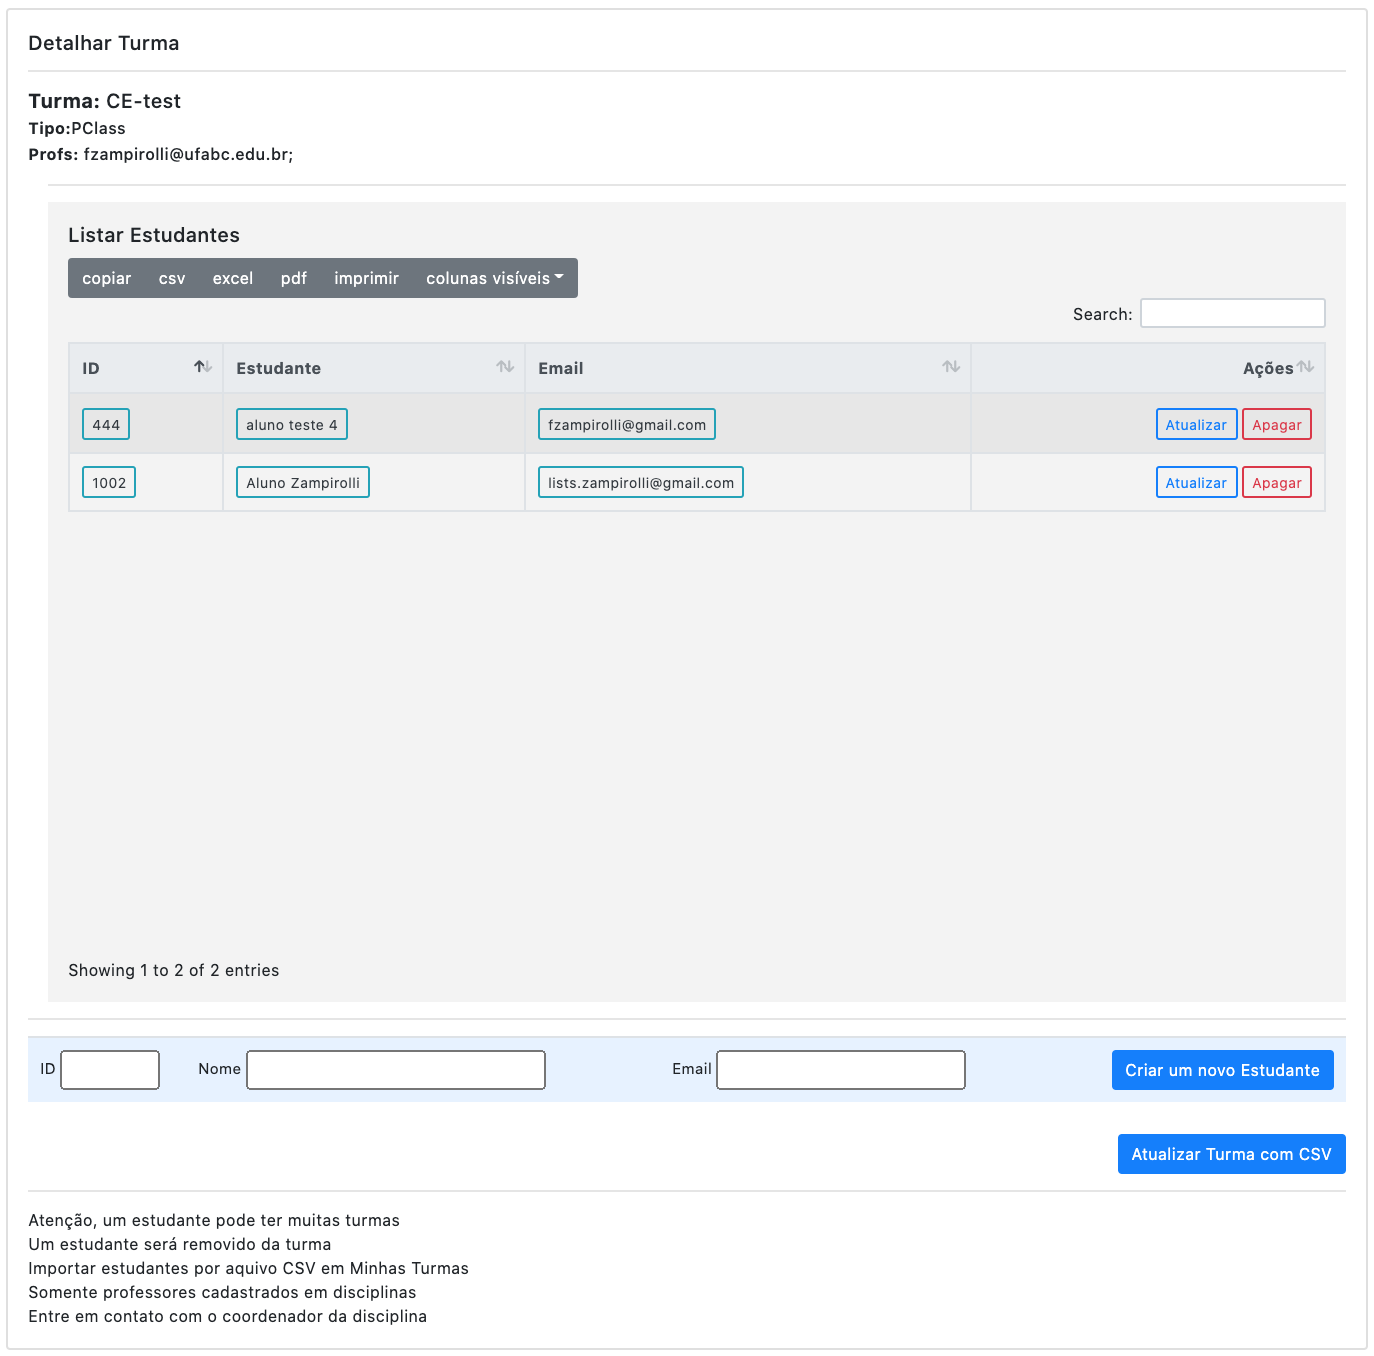
\includegraphics[width=0.9\textwidth]{cap02_figTurmaAtualiza2.png}
  \caption{Tela para um professor de uma disciplina poder atualizar uma turma, atualizando ou apagando estudantes da turma. Além disso, é possível incluir um novo estudante na turma.}
  \label{fig:cap02_figTurmaAtualiza2}
\end{figure}

Além disso, ao clicar no nome de um estudante específico, o professor pode acessar a tela apresentada na Figura \ref{fig:cap02_figTurmaAtualiza3}, onde é possível atualizar os dados do estudante, como nome, e-mail e matrícula. Essa funcionalidade permite que os professores mantenham a lista de estudantes atualizada e corrigir eventuais erros ou inconsistências nas informações.

\begin{figure}[!ht]
  \centering
  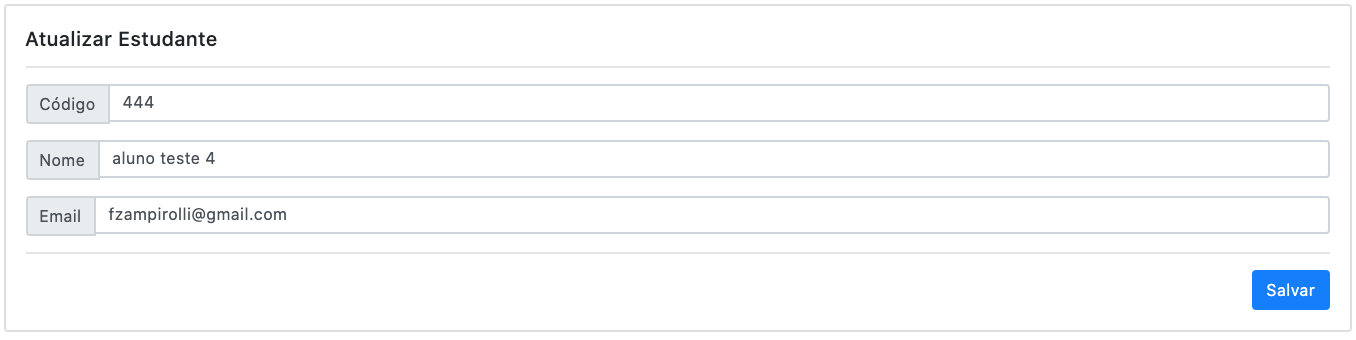
\includegraphics[width=0.9\textwidth]{cap02_figTurmaAtualiza3.png}
  \caption{Tela para um professor de uma disciplina poder atualizar os dados de um estudante da turma.}
  \label{fig:cap02_figTurmaAtualiza3}
\end{figure}

% \newpage

% \ \\ \ 

% \newpage

% \ \\ \ 

% \newpage

\subsection{Tópico}\label{sec:topicos}

Os tópicos são definidos para agrupar questões numa disciplina. Cada disciplina possui um conjunto de tópicos associados. A criação, atualização ou exclusão de um tópico de disciplina(s) é restrita ao usuário com perfil de coordenador ou ao administrador, conforme indicado na lista de tópicos apresentada na Figura \ref{fig:cap02_figTopico}. É importante ressaltar que a lista exibida corresponde aos tópicos das disciplinas onde o usuário está envolvido.


\begin{figure}[!ht]
  \centering
  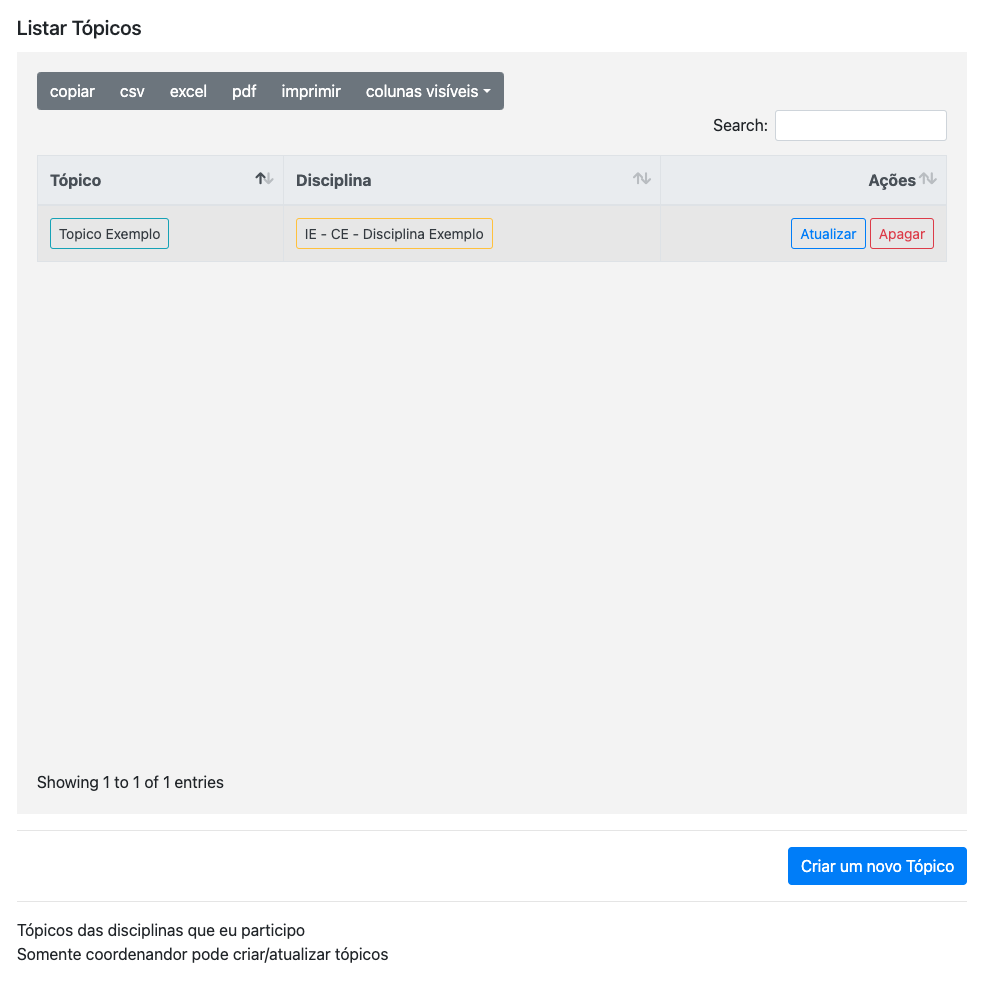
\includegraphics[width=0.9\textwidth]{cap02_figTopico.png}
  \caption{Tela com a lista de tópicos para o coordenador (ou administrador) criar, atualizar ou apagar um tópico de disciplina(s).}
  \label{fig:cap02_figTopico}
\end{figure}

A Figura \ref{fig:cap02_figTopicoAtualiza} apresenta a tela para atualização de um tópico, que é semelhante à tela de cadastro de um novo tópico. Uma das principais funcionalidades disponíveis nessa tela é a possibilidade de associar mais de uma disciplina ao tópico em questão, mantendo a tecla \texttt{Ctrl} pressionada. Essa flexibilidade permite que um mesmo tópico possa ser utilizado em diferentes disciplinas, conforme as necessidades e particularidades de cada uma delas.

\begin{figure}[!ht]
  \centering
  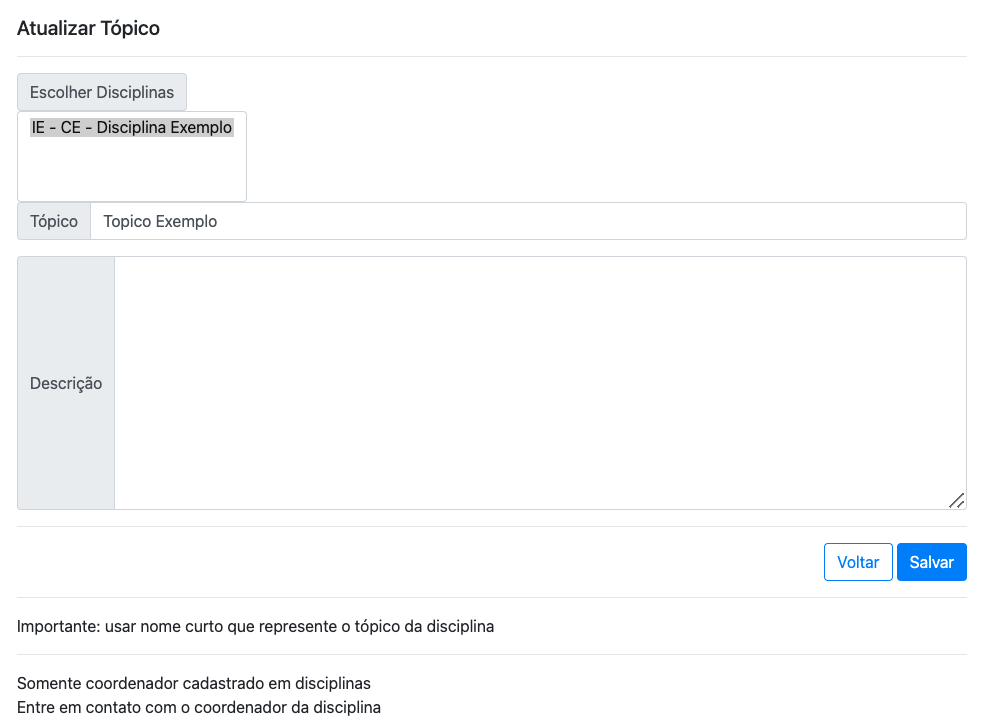
\includegraphics[width=0.9\textwidth]{cap02_figTopicoAtualiza.png}
  \caption{Tela para o coordenador (ou administrador) atualizar um tópico de uma disciplina.}
  \label{fig:cap02_figTopicoAtualiza}
\end{figure}

Ao clicar em um tópico na primeira coluna da Figura \ref{fig:cap02_figTopico}, será aberta uma tela detalhando as questões relacionadas ao tópico, conforme ilustrado na Figura \ref{fig:cap02_figTopicoDetalha} (as outras colunas serão detalhadas nos próximos capítulos). É importante destacar o botão ``Criar-PDF'', que permite a criação de um arquivo PDF contendo todas as questões do tópico selecionado, conforme ilustrado na Figura \ref{fig:cap02_figTopicoDetalha2}. Detalhes sobre este arquivo serão abordados em capítulos futuros.

\begin{figure}[!ht]
  \centering
  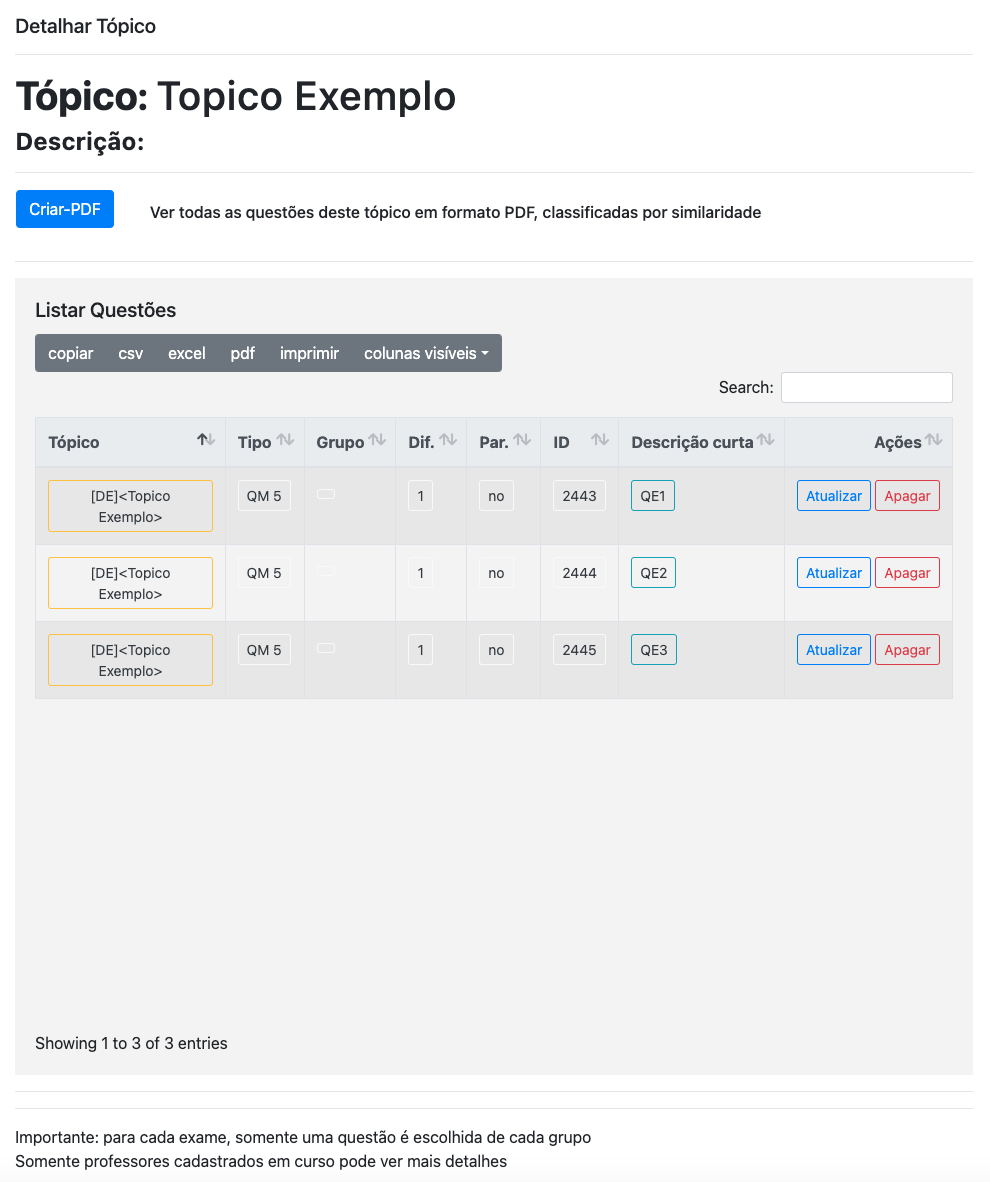
\includegraphics[width=0.9\textwidth]{cap02_figTopicoDetalha.png}
  \caption{Tela apresentando os detalhes de um tópico.}
  \label{fig:cap02_figTopicoDetalha}
\end{figure}

\begin{figure}[!ht]
  \centering
  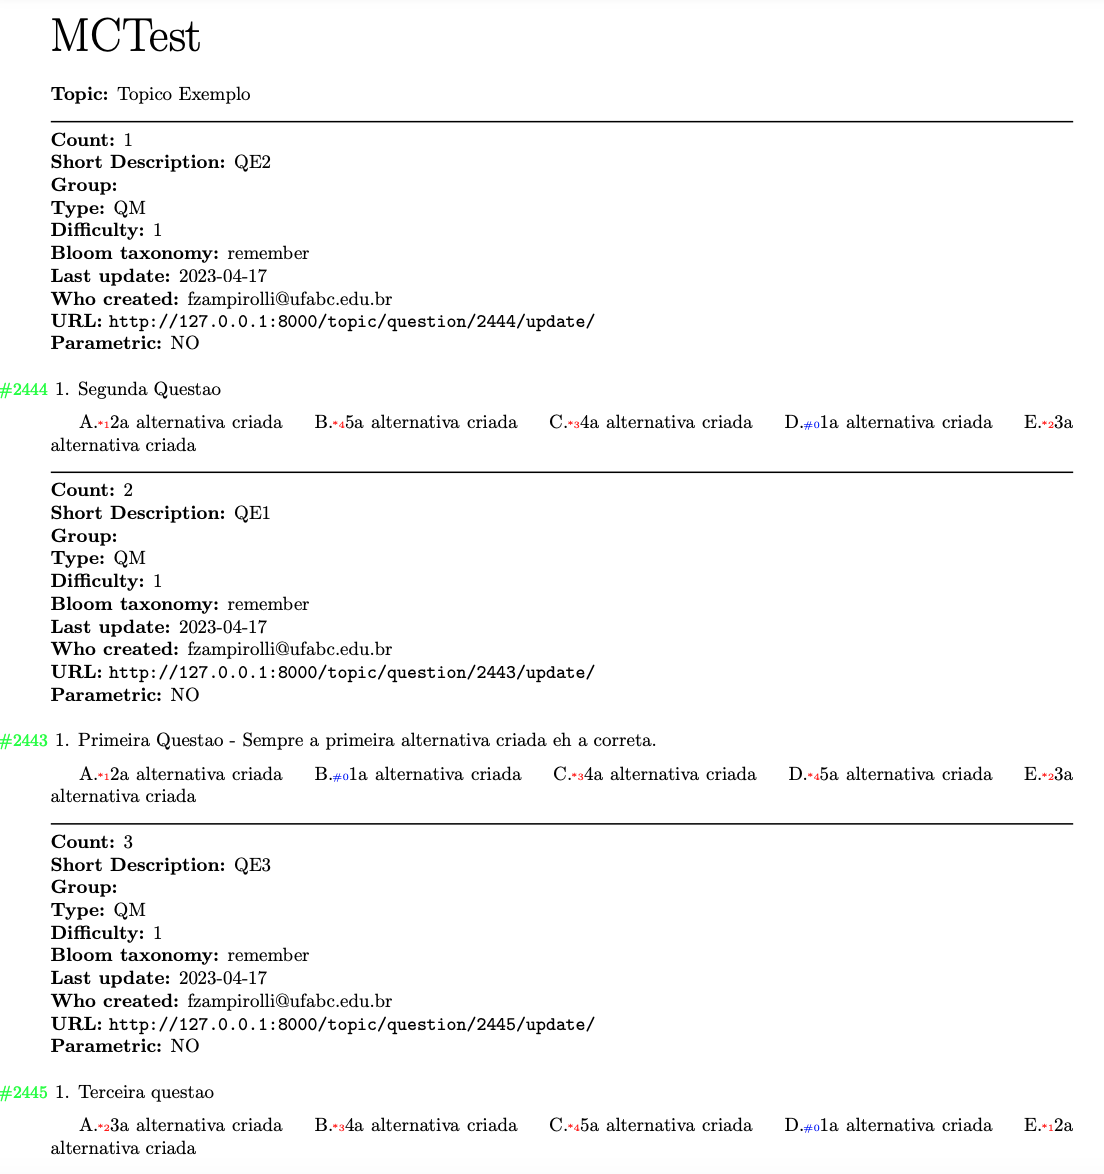
\includegraphics[width=0.9\textwidth]{cap02_figTopicoDetalha2.png}
  \caption{Tela apresentando as três primeiras questões de um tópico.}
  \label{fig:cap02_figTopicoDetalha2}
\end{figure}

% \newpage

% \ \\ \ 

% \newpage

% \ \\ \ 

% \newpage

% \ \\ \ 

% \newpage

\section{Considerações finais}

Neste capítulo, foi apresentada uma visão geral do MCTest, enfatizando sua estrutura e funcionalidades essenciais. Foi discutida a navegação geral do sistema, destacando como os usuários podem acessar as diferentes entidades disponíveis, como institutos, cursos, disciplinas, turmas e tópicos.

Os diferentes tipos de usuários com acesso ao MCTest foram apresentados, incluindo administrador, coordenador e professor, juntamente com suas respectivas permissões e responsabilidades específicas.

O administrador foi identificado como o usuário com maior privilégio, possuindo acesso irrestrito a todas as funcionalidades e dados do sistema. Sua responsabilidade abrange a configuração do sistema, criação e gerenciamento de outros usuários, bem como a definição de parâmetros gerais do MCTest.

O coordenador, por sua vez, possui um conjunto de ferramentas específicas para gerenciar a disciplina, permitindo a criação e manutenção de tópicos relevantes para o andamento das aulas, bem como a criação de turmas e seus respectivos estudantes. É importante ressaltar que o acesso às configurações gerais do sistema é restrito ao administrador. Além disso, o coordenador pode cadastrar outros coordenadores e professores para colaborarem na gestão da disciplina. Uma funcionalidade interessante disponível ao coordenador é a criação de turmas por meio da importação de arquivos CSV, prática que favorece a organização e evita possíveis erros durante a inserção manual de dados.

O professor tem acesso mais restrito em comparação com o coordenador e o administrador. Sua responsabilidade abrange a criação e manutenção dos exames, turmas e estudantes atribuídos a ele, assim como a elaboração e utilização de questões da disciplina. No entanto, ele não possui permissão para cadastrar ou editar disciplinas, ou tópicos, reservadas ao coordenador e ao administrador. 

Os detalhes específicos de cada funcionalidade atribuída a esses usuários serão abordados em capítulos futuros, fornecendo informações detalhadas sobre as ferramentas disponíveis para cada perfil, bem como as ações que podem ser realizadas no sistema.

As entidades questão e exame desempenham papéis fundamentais no MCTest, e suas descrições detalhadas serão realizadas nas Partes \ref{part:questoesMCTest} e \ref{part:exames}, respectivamente. %Isso ocorre devido às suas complexidades e relevâncias para o funcionamento do sistema.

A elaboração de questões parametrizadas representa o aspecto mais desafiador do sistema, exigindo criatividade, conhecimento da sintaxe \LaTeX{} e domínio da linguagem Python. No entanto, após a criação bem-sucedida dessas questões, elas podem ser reutilizadas em diversos exames, desde que adequadamente parametrizadas. Essa característica simplifica a criação de novos exames.

A entidade exame, por sua vez, é considerada o elemento central do sistema, uma vez que todo o processo avaliativo é construído em torno dela. Os exames representam a ferramenta por meio da qual os estudantes são avaliados e os resultados obtidos, tornando essa entidade indispensável para o êxito do MCTest como um sistema de avaliação educacional.